% (C) Anders Kofod-Petersen
\documentclass[a4paper]{book}
\usepackage[english]{babel}						% Correct English hyphenation
\usepackage[latin1]{inputenc}						% Allow for non-English letters
\usepackage{graphicx}							% To include graphics
\usepackage{subfig}
\usepackage[square,numbers, sort&compress,numbers]{natbib}
\bibliographystyle{unsrtnat}
%\bibliographystyle{apalike}
%\bibpunct{[}{]}{;}{a}{,}{,}	
% Correct citations
%\usepackage{fancyheadings}						% Nice header and footer
\usepackage[linktocpage,colorlinks]{hyperref}			% PDF hyperlink
\usepackage{geometry} 							% Better geometry
%\usepackage[center]					% For cropping documents
\usepackage{amsmath}
% B5 (uncomment to convert to B5 format)
 \geometry{b5paper}

% Author
% Fill in here, and use commands in the text. 
\newcommand{\thesisAuthor}{Johan Phan}
\newcommand{\thesisTitle}{Batch-incremental method in Active Learning for image classification}
\newcommand{\thesisType}{Master project}
\newcommand{\thesisDate}{Winter 2018}

% PDF info
\hypersetup{pdfauthor={\thesisAuthor}}
\hypersetup{pdftitle={\thesisTitle}}
\hypersetup{pdfsubject={\thesisType}}
\hypersetup{linkcolor=black}
\hypersetup{citecolor=black}
\hypersetup{urlcolor=black}

%Fancy headings
%\pagestyle{fancy}
%\pagestyle{fancyplain}
%\renewcommand{\chaptermark}[1]{\markboth{#1}{}}
%\renewcommand{\sectionmark}[1]{\markright{#1}{}}
%\lhead[\fancyplain{}{\thepage}]{\fancyplain{}{\let\uppercase\relax\leftmark}}
%\rhead[\fancyplain{}{\let\uppercase\relax\rightmark}]{\fancyplain{}{\thepage}}
%\chead[\fancyplain{}{}]{\fancyplain{}{}}
%\lfoot[\fancyplain{}{}]{\fancyplain{}{}}
%\cfoot[\fancyplain{}{}]{\fancyplain{}{}}
%\rfoot[\fancyplain{}{}]{\fancyplain{}{}}

% Citation format

\begin{document}
%Title page (This is generate automatically from the commands above)
\begin{titlepage}
\noindent {\large \textbf{\thesisAuthor}}
\vspace{2cm}\\
\noindent {\Huge \thesisTitle}
\vspace{2cm}\\
\noindent \thesisType, \thesisDate 
\vspace{1cm}
\noindent \\ Supervisor: Massimiliano Ruocco \\
\noindent Co-supervisor: Francesco Scibilia\\
\vspace{1cm}
\noindent \\Department of Cybernetics Engineering\\ Faculty of Information Technology, Mathematics and Electrical Engineering\\
\vfill
\begin{center}

\includegraphics[width=3cm]{Image/NTNUlogo.pdf}
\end{center}
\end{titlepage}

\thispagestyle{empty}

\cleardoublepage

\frontmatter

\section*{Abstract}
In the recent year, Deep Learning has seen a rapid surge of interest across academia and industry. One of the main factor that contribute to the rise of Deep Learning is the successful applications of convolutions neural network by using very deep and advance model like VGG-net and  Res-Net image.
However, in order to effectively utilize the power of it, we still need to gather a large amount of data, especially labeled data, which sometimes require an expert to do the task. On the other hand, unlabeled has become much cheaper and easier to obtain and because of that, active learning has become one of the main approach to reduce labeling cost without scarifying performance. In this report, we will look at the current state of the art works in active learning and compare their performance on a pre-trained deep convolutional network. ++++

\clearpage

\section*{Preface}



\vspace{1cm}
Thanks ABCXYZ\\
Supervisor:  Massimiliano Ruocco\\
Co-supervisor:  Francesco Scibilia

The preface includes the facts - what type of project, where it is conducted, who supervised and any acknowledgements you wish to give. 

\vfill

\hfill \thesisAuthor

\hfill Trondheim, \today

\clearpage

\tableofcontents

\listoffigures

\listoftables

\mainmatter

\chapter{Introduction}
\label{cha:Introduction}
Image classification using machine learning has recently enjoyed a great degree of success thanks to Deep learning and Convolutional Neural Network. One of the main factor that contributed to this success is the rise of big data where huge data-set can be use to train the learner. As for supervised learning tasks, Deep Convolutional Neural Network required thousands, if not tens, hundreds of thousands labeled data in order to deliver desired results. This intensive demands of labeled data is still remain one of the biggest challenge in Deep Learning today, especially in cases where we need expert to do the labelling work e.g MRI scans. Due to the fact that unlabeled data is normally much easier to obtain then labeled data, active learning has become one of the primary approach to reduce the labeling effort without scarifying the performance. The essence of active learning is, given a large unlabeled data pool, the active learner will select "the highest quality" instances to be labeled by an oracle. In this way, the active learner aims to achieve best performance in term of accuracy using as small labeled data set as possible, thereby reducing the labeling cost. 
In this report, we will take a look at the current state of the art methods in active learning for deep convolutional neural network and compare their performance on different data sets . This report is means to provide the reader an overview of active learning using batch-mode approach and the experiment will be conduct on a VGG-16 model with pretrained weights on the popular ImageNet database.


\section{Background and Motivation}\label{cit}

\label{sec:BackgroundAndMotivation}
Studies around active learning has started even before the rise of deep learning, in \citet{tong2001active}, experiments and discussion based on the performance of active learning on support vector machine(SVM) has been address and thoughtfully studied. However in the last decade, follow the success of deep learning and the abundance of unlabeled data thanks to the internet, the interest in active learning has become larger than ever. 
-need more background ----

Serial-mode active learning is a method that the active learner can only query a single instance at a time has been intensively studied in the last recent years and achieved a great degree of success \citet{activelearningbook}. However, such method is very impractical for real world application where the oracle labelling speed is normally much faster than the system query speed, since a modern deep learning model requires a signification amount of time to train. In order the utilize the power of active learning in real world application, batch-mode active learning has been proposed as a solution for this problem. In batch mode active learning, the learner will select a set of instances and perform query batch by batch. 
++++ next next
In \citet{activelearningbook}, the author has mentioned 
+++++
+++++
Todo- motivation 


\section{Goals and Research Questions}
\label{sec:Goals and Research Questions}
This project is meant to study the potential of using active learning in real world application where labeled data is very expensive to obtain. Therefore the first goal of this work is to provide the reader an overview of different recent state of the art approaches in batch-mode active learning for image classification problem and compare their performance on different setting and different data set. Additionally, we also want to address different problem with batch-mode active learning and study how incremental learning will affect the performance of active learning. In this report, we will to try to answer the following research questions:

\begin{description}
\item[Research question 1] {\it hmmm???   }
\end{description}

\begin{description}
\item[Research question 2] {\it How different selection criteria will affect the performance of the classification model in term of accuracy per labeled instances? }
\end{description}



{\it Lorem ipsum dolor sit amet, consectetur adipiscing elit. Nam consequat pulvinar hendrerit. Praesent sit amet elementum ipsum. Praesent id suscipit est. Maecenas gravida pretium magna non }

\section{Research Method}
\label{sec:researchMethod}
In this Research, we will compare different mode of active learning with random selection of the data set.




\section{Report Structure}
\label{sec:reportStructure}
The rest of the report is organized as follows. 
Chapter 2 is an introduction to some of the basic concept in deep learning and active learning. The chapter will also address some of the related work in the active learning for image classification field. Chapter 3 outlines how different method of active learning is going to be implement in the experiments. In chapter 4, we will go though the experiments process and it result will be show for further discussion in chapter 5.

\chapter{Background Theory and Related work}\label{T-B}
\label{cha:TheoryAndBackground}

In this chapter, we will go through diffirent 


\section{Background Theory}


\subsection{Image classification using Convolutional Neural Networks }
As one of the biggest contributing factor to the rise of Deep learning, Convolutional neural network(CNN) (LeCun et al., 1998) has become the most dominant player in the field of image classification. The interest in CNN started with Alexnet(2012)\cite{CNN} which scored a top-5 accuracy of 15.3\% on the ImageNet competition\cite{ILSVRC15}, which was 10.8 percentage points lower than that of the runner up. Since then, the architecture of CNN has changed a lot, with deeper and more powerful performance. 
\begin{figure}[ht]
\begin{center}
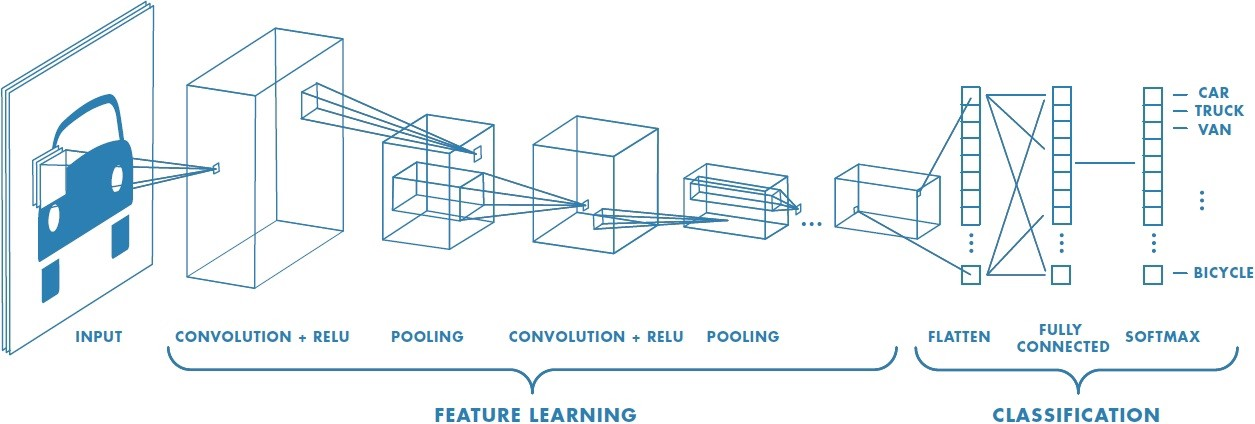
\includegraphics[width=0.5\columnwidth]{Image/CNN.jpeg}
\caption[CNNpic1]{ Basic convolutional neural network architecture \cite{CNNpic}}
\label{fig:BoxesAndArrowsAreNice}
\end{center}
\end{figure}

In short, convolutional networks are a subset of neural networks, they are also made up of neurons that have learnable weights and biases. In CNN, the network will process the input train data through a series of convolution layers with filters (Kernals), Pooling, fully connected layers (FC), etc... and then perform the classification with help of function like softmax at the end.\cite{CNN} Convolution in this case is the first layers of the network, which apply filters to the input tensor. It can extract the features from the image by preserving the relation between pixels. The pooling layer then use to reduce the numbers of parameters, which is very useful for example when the input image is large. 
\subsubsection{VGG-net}
The VGG-net is a deep convolutional neural network for object recognition developed and trained by  Visual Geometry Group from Oxford.\cite{2014arXiv1409.1556S} "It was demonstrated that the representation depth is beneficial for the classification accuracy, and that state-of-the-ar performance on the ImageNet challenge dataset can be achieved using a conventional CNN architecture with substantially increased depth. " (VGG-net authors)
Until today, VGG-net still remain one of the most cost-effective CNN- architecture because of the short required training and it relative powerful performance.

\begin{figure}[ht]
\begin{center}
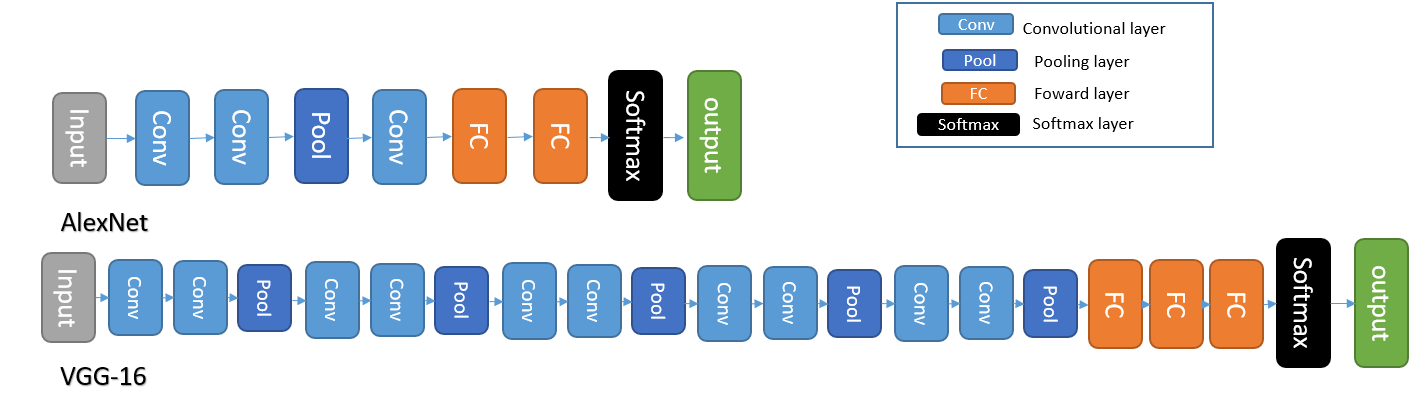
\includegraphics[width=1\columnwidth]{Image/alexvgg.PNG}
\caption[CNNpic1]{ Architecture Comparition between Alexnet and VGG-16  \cite{CNNpic}}
\label{fig:BoxesAndArrowsAreNice}
\end{center}
\end{figure}

\subsection{Active learning}
Even with the most advance neural network architecture, it is still impossible to achieve a acceptable result without a sufficient amount of labeled data. However, the acquisition of labeled data for new tasks is both challenging and costly. In such case, active learning can be used to lower the cost of annotation without sacrificing. The motivation behind active learning focus on, given a pool of unlabeled data and a limited annotation-budget, there must exist an optimal way to query the best sub-set of it for label, such that sub-set queried by active learning would significantly outperform a random selected sub-set. The problem of active learning in image classification can be formulated as follow. Given  an unlabeled data-set of $X^U$ and a labeled data-set of $X^L$ , the algorithm need to take $k$ samples from $X^U$, query the correspond label from an oracle and add them to $X^L$ in order to minimize the classification error of a model trained on $X^L$.
\subsection{Batch-mode Active learning}
In most active learning research, the queries are selected one at a time, i.e serial. However, such method is sometimes very very inefficient and time-consuming \cite{activelearningbook}. In many cases, there would be multiple annotators working on different labeling workstations at the same time span on a network and the query speed is not fast enough to catch up with the labeling speed. In such cases, active learning method that selecting queries in serial may be inefficient and this has given rise to batch-mode active learning. Batch-mode active learning allow the learner to query instances in groups, which proof to be more effective for parallel labeling or network with long training time. The goal of batch-mode active learning is to select an optimal query set $\mathbf{Q}$ which performance is comparable with serial selecting. Although, it is very challenging since the active learner fails to consider the overlap in information content among the selected instances and for batch. There has been several research studies that address this problem \cite{Discriminativebatchmode} and various of proposed method to combat this \cite{6912976}. For the most part, these approaches has show a better result then random batch sampling, but still not comparable to serial query. \cite{activelearningbook}
\subsection{Active learning in image classification}
Active learning has been applied and achieved a considerable amounts of success in different area of machine learning, from speech recognition to object detection \cite{workshop}. As for image classification, the key idea of active learning revolve around achieve greater accuracy with fewest number of labeled training samples. One of the most common approach is uncertainty base active learning, where the learner select instances based on the classifier uncertainty. However, we can also perform selection base on dissimilarity between instances, i.e distances between data points or by reducing the expected error reduction by simulate the label outcome of each instances. 


\subsection{Uncertainty base active learning}
One of the most basis and simplest method in active learning is to query base on the uncertainty of the classifier. For this method there are 3 main way to determine the selection criteria: Least confidence (LC), margin sampling (MS) \cite{roy2001toward}, and entropy \cite{shannon1948mathematical}. 
\subsubsection{Least confidence selection}
This method query instances one by one by select the unlabeled instances $x_i$ that have lowest score given by the function $max(p(y_j|x_i))$, which is the probability of instance $x_i$ belongs to class $y_j$.
\begin{equation}
    x^{LC}_i =\underset{x \in X^U}{argmin} ( max(p(y_j|x_i)))
\end{equation}
\subsubsection{Margin sampling selection}
This strategy pick the sample with the smallest probability different of the top two class predictions $y_1$ and $y_2$.
\begin{equation}
    x^{MS}_i =\underset{x \in X^U}{argmin} ( (p(y_1|x_i)- p(y_2|x_i)))
\end{equation} 
\subsubsection{Entropy selection}
The selection takes all class label probabilities into consideration to measure uncertainty and select the one with largest class prediction information entropy.
\begin{equation}
    x^{entropy}_i =\underset{x \in X^U}{argmax} (\sum_{j}p(y_j|x_i)log(p(y_j|x_i))
\end{equation} 
\subsection{Deep Bayesian Active Learning}
Deep Bayesian Active Learning(BALD) \citet{GalIG17}, is one of the more sophisticated uncertainty base method of active learning designed for deep CNN. The method make use of the Bayesian equivalent of CNN\citet{gal2015bayesian}, which are CNNs with prior probability distribution placed over a set of model parameters $\omega = {W_1, ... , W_L}$. To achieve this, we applied stochastic regularization techniques such as dropout where dropout can be interpreted as a variational Bayesian approximation. The prediction probabilities of an instance in this case will be:
\begin{equation}
    p(y_j|x_i) = \frac{1}{T} \sum_{t=1}^Tp(y_j|x_i, \hat{\omega}_t)
\end{equation} 
with T is the number of different outcome of the neural network affected by $\hat{\omega{_t}}$ with $\hat{\omega{_t}} \sim q^{*}_\theta(\omega)$ where  $q^{*}_\theta(\omega)$ is the dropout distribution. The selection function of this method can be written as follows:
\begin{equation}
    x^{BALD}_i =\underset{x \in X^U}{argmin} (- log(p(y_j|x_i)) + \frac{1}{T}\sum_{t=1}^Tp(y_j|x_i,\hat{\omega}_t)log(p(y_j|x_i,\hat{\omega}_t)))
\end{equation}
where $p(y_j|x_i, \hat{\omega}_t)$ is the prediction probability of each CNN with different weight parameters affected by dropout.  
\subsection{Deep Bayesian Active Learning}    
\subsection{Cost-effective active learning}
\begin{equation}
    S^{A}_{x} = \begin{bmatrix}
       |5| \\[0.3em]
       \frac{5}{6} \\[0.3em]
       0           
     \end{bmatrix}
\end{equation}
\subsection{Criteria switching active learning}
As previous mentioned, active learning is st 
\begin{figure}[ht]
\begin{center}
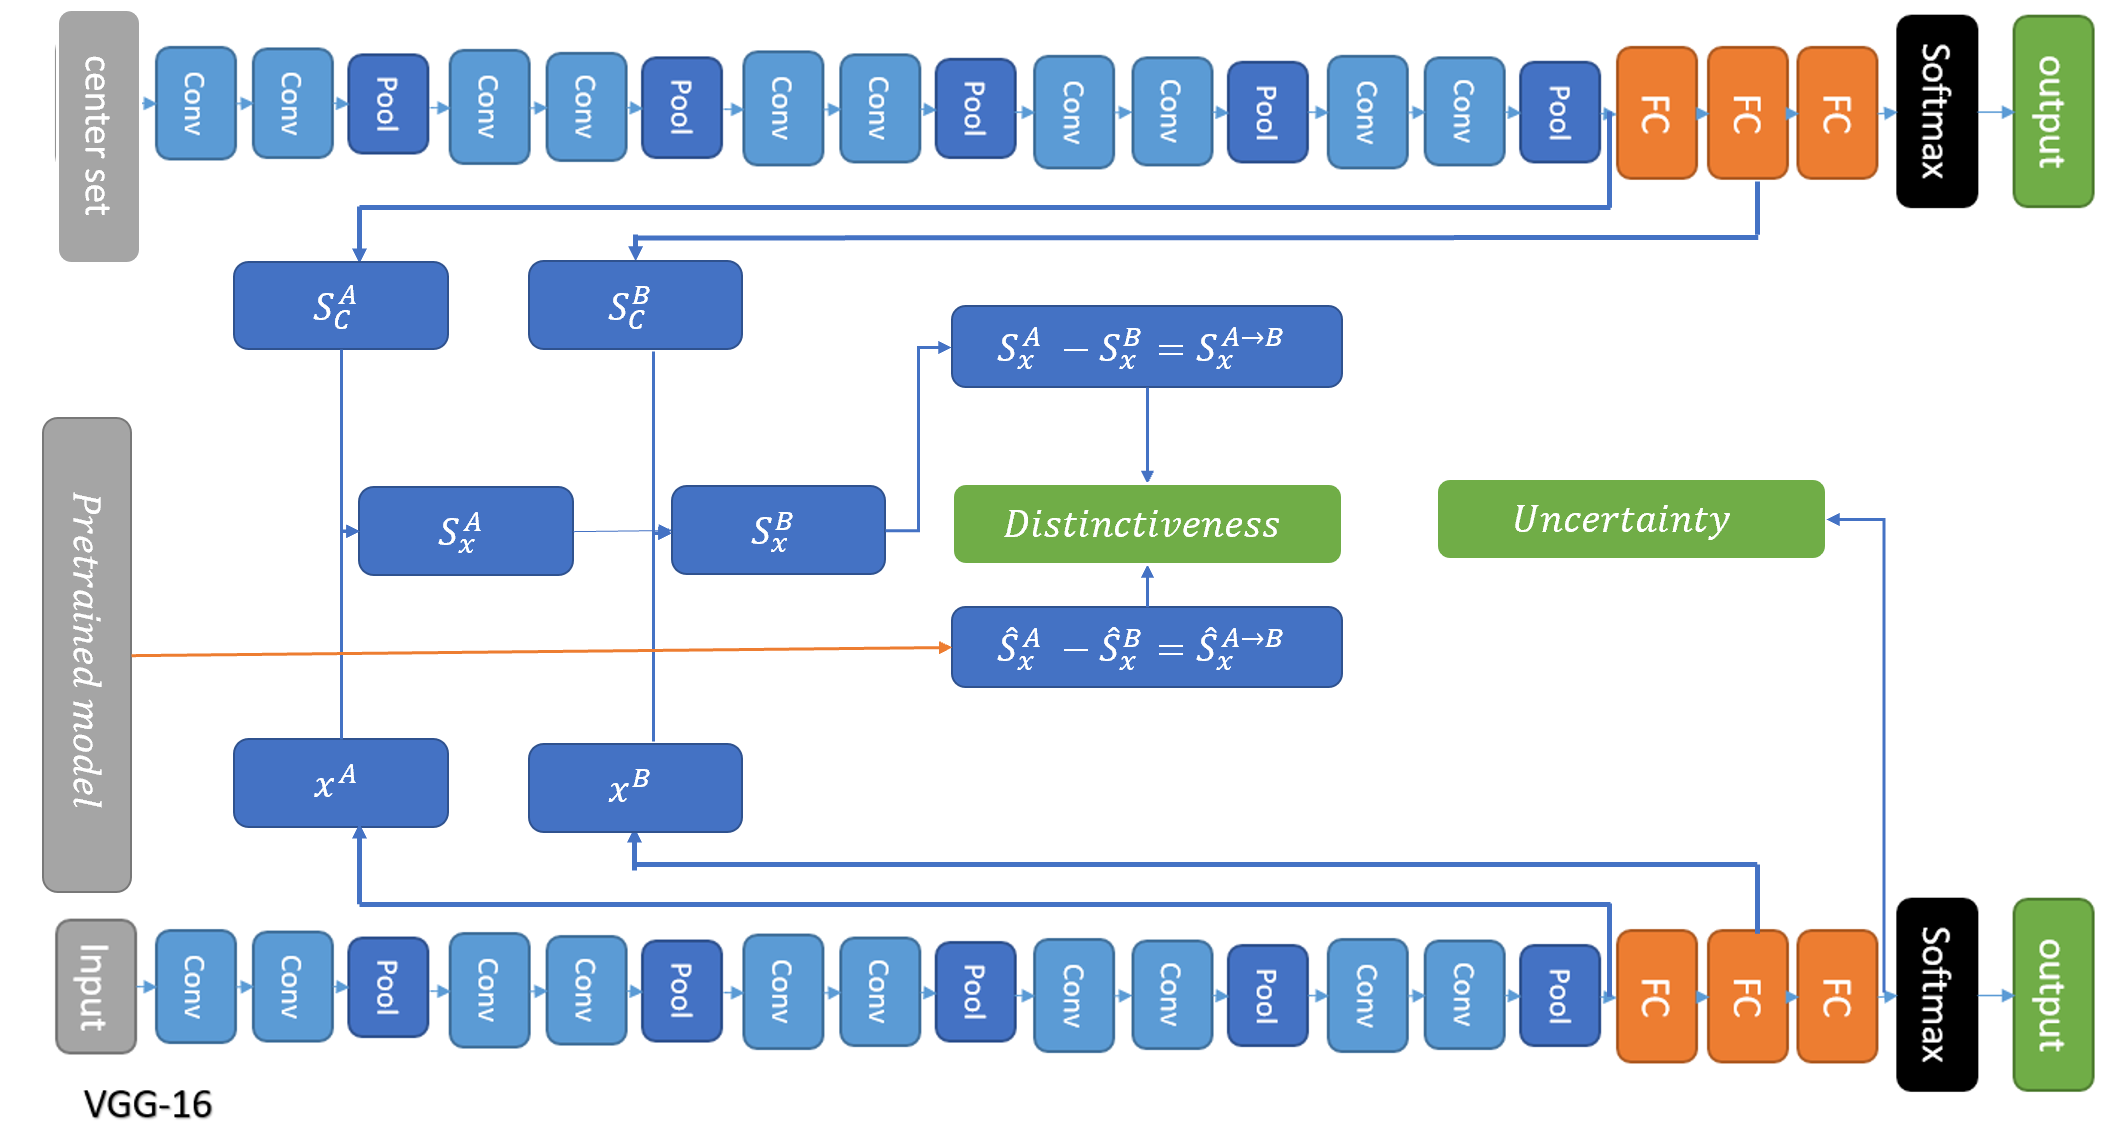
\includegraphics[width=1\columnwidth]{Image/vgg.PNG}
\caption[vgg]{ cost effective }
\label{fig:BoxesAndArrowsAreNice}
\end{center}
\end{figure}
\cite{costeffective}
\cite{costeffective2}
\subsection{Core-set approach Active learning}
\label{sec:no1}

%The background theory depth and breadth depends on the depth needed to understand your project in the different disciplines that your project crosses.  It is not a place to just write about everything you know that is vaguely connected to your project. The theory is here to help the reader that does not know the theoretical basis of your work so that he/she can gain sufficient understanding to understand your contributions. In particular, the theory section provides an opportunity to introduce terminology that can later be used without disturbing the text with a definition.  In some cases it will be more appropriate to have a separate section for different theory. However, watch that you don't end up with too short sections. Subsections may also be used to separate different background theory. 

%When introducing techniques or results, always reference the source. Be careful to reference the original contributor of a technique and not just someone who happens to use the technique. For relevant results to your work, you would want to look particularly at newer results so that you have referenced the most up-to-date work in your area. If you don't have the source handy when writing, mark the test that a reference is needed and add it later. 

%Web pages are not reliable sources --- they might be there one day and removed the next; and thus should be avoided, if possible. A verbal discussion is not a source and should not be referenced or described in the text.  

%The bulk of citations in the report will appear in section~\ref{cit}. However, you will often need to introduce some terminology and key citations already in this chapter. 

%You can cite a paper in the following manners: 



\noindent
{\bf Introducing tables in the report: }\\

\begin{table}[htbp]
\begin{center}
\begin{tabular}{|c|c|c|c|c|}\hline\hline
This & is & a & nice & table\\\hline
This & is & a & nice & table\\\hline\hline
\end{tabular}
\caption{Example Table}
\end{center}
\label{tab:ExampleTable}
\end{table}%

As you can see from Table \ref{tab:ExampleTable}, tables are nice. However, again, you need to discuss the contents of the table in the text. You don't need to describe every entry but draw the authors attention to what is important for he/she to glean from the table. 

\section{Structured Literature Review Protocol}

What is this ???

\section{Related work}
\label{sec:no2}

\subsection{Uncertainty base active learning}
\subsection{Distance base active learning}
\subsection{Cost-effective active learning}

\chapter{Model and PROPOSED APPROACH}
\label{sec:architectureAndModel}
\section{Classifier model}
In this work, a pretrained VGG-16 model has been chosen as the base classifier. However, We only use pretrained weight on the convolution part of the pretrained model. The VGG-16 is chosen because it is fast to run and the out accuracy is also acceptable. 
\section{Active learner model}
\subsection{Least confident approach}
\subsection{Least confident approach}
\subsection{K-greedy approach}
As a part of 
\subsection{Cost-effective approach}



Here you will present the architecture or model that you have chosen and that is (or will be) implemented in your work. Note that putting algorithms in your report is not desirable but in certain cases these might be placed in the appendix. Code further be avoided in the report itself but may be delivered in the fashion requested by the supervisor or, in the case of masters delivery, submitted as additional documents. 

\chapter{Experiments and Results}
\label{cha:ResearchAndResults}

Result 1: random vs cost effective batch mode active learning, batch size of 200. 10000 epochs 
Result 2: Comparison of active learning 

Current plan
Random Sampling
Least Confidence [1]
Margin Sampling [1]
Entropy Sampling [1]
Uncertainty Sampling with Dropout Estimation [2]
Bayesian Active Learning Disagreement [2]
K-Means Sampling [3]
K-Centers Greedy [3]
Core-Set [3]
Adversarial - Basic Iterative Method
Adversarial - DeepFool [4]
\section{Experimental Plan}
\label{sec:experimentalPlan}
In the experiments, we want to study how batch incremental method of active learning works on the cifar-10 data-set and the data-set. For the classification model, we choose to use the VGG-net because it simplicity, short training time and powerful performance. The experiment will by conducts using Pytorch which is one of the most popular deep learning platform. 
The plan is first to compare the performance of different uncertainty base method. Then try the same thing with distance base method and BALD.



\section{Experimental Setup}

\label{sec:experimentalSetup}
For the first experiment, the active learner will query 100 instances for every 10 epoch of training. The training process will happens incrementally, where the size of the training set will gradually increase. Nearly all of the weight in the VGG-net will be initialized by using pre-trained weight, expect for the last three forward fully connected layer. The pre-trained weight is loaded from a pre-trained VGG model of ImageNet data-set which consist of 150,000 photographs and  1000 classes.




Optimizer Adam:
learning rate 0.0001, 
betas=(0.9, 0.999),
eps=1e-08, 

Graph1
Graph2
Graph3 making
\section{Experimental Results}

\label{sec:experimentalResults}
\subsection{Uncertainty base active learning}
\begin{figure}[!htb]%
    \centering
    \subfloat[]{{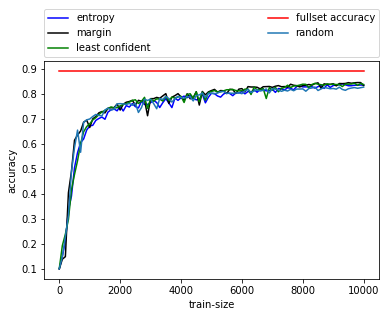
\includegraphics[width=5cm]{Contens/results/confident.png} }}%
    \qquad
    \subfloat[]{{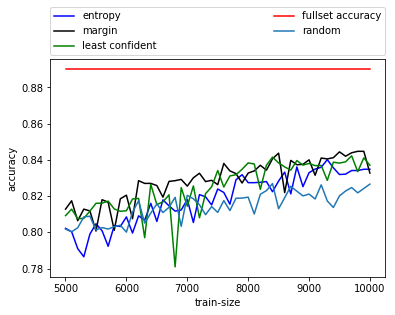
\includegraphics[width=5cm]{Contens/results/confident2.png} }}%
    \caption{Uncertainty base}%
    \label{fig:uncertainty1}%
\end{figure}
\subsection{BALD}

\begin{figure}[!htb]%
    \centering
    \subfloat[]{{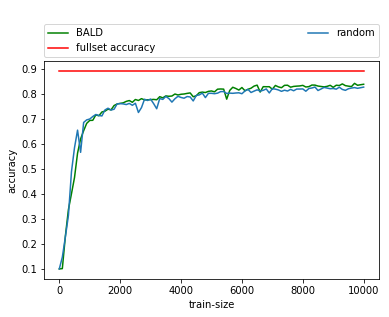
\includegraphics[width=5cm]{Contens/results/Bald1.png} }}%
    \qquad
    \subfloat[]{{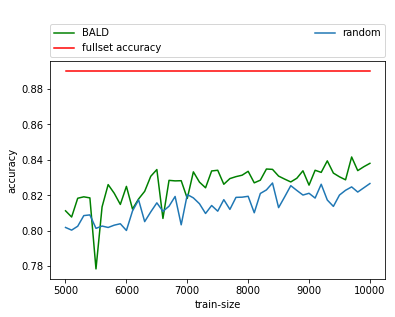
\includegraphics[width=5cm]{Contens/results/Bald2.png}.png} }%
    \caption{BALD}%
    \label{fig:BALD}%
\end{figure}
\subsection{Uncertainty base active learning}

Results should be clearly displayed and should provide a suitable representation of your results for the points you wish to make. Graphs should be labeled in a legible font and if more than one result is displayed on the same graph then these should be clearly marked.   Please choose carefully rather than presenting every results. Too much information is hard to read and often hides the key information you wish to present. Make use of statistical methods when presenting results, where possible to strengthen the results.  Further, the format of the presentation of results should be chosen based on what issues in the results you wish to highlight. You may wish to present a subset in the experimental section and provide additional results in the appendix.
\subsection{Least Confidence }
\subsection{Entropy Sampling}



\chapter{Evaluation and Conclusion}
\label{cha:evaluationAndConclusion}



\section{Evaluation}
\label{sec:Evaluation}
\subsection{Uncertainty base method}
In  Figure \ref{fig:uncertainty1} we can see that in the grand scale, in the uncertainty base methods behave similarly with random method, however when we looks closer at the half end of the left figure, most of the uncertainty base method gives 1\% improvement in accuracy compare with the random method.   

In this experiment, we have tried to advoid the use of core-set and adversarial approaches 
%When evaluating your results, avoid drawing grand conclusions, beyond that which your results can in fact support. Further, although you may have designed your experiments to answer certain questions, the results may raise other questions in the eyes of the reader. It is important that you study the graphs/tables to look for unusual features/entries and discuss these as well as discussing the main findings in the results. 
\subsection{Distance based method}:
In this project, we have also tried to apply the core set 
\section{Discussion}
\label{sec:Discussion}
\section{Uncertainty base active learning and Bald}
Most of the uncertainty base active learning suffers heavily when run batch incremental mode. It is not a surprise since for large batch size, the instances that give the same uncertainty output tends to belong to the same class or very similar to each other. Because of this overlapping, the uncertainty base active learner will not able to query instances in a diversify manner, which lead to poorer performance. 
\subsection{The effect of batch-size during incremental learning}
In  Figure \ref{fig:uncertainty1} we can see 


\section{Contributions}~\label{cont}
\label{sec:Contributions}
For the situation where we gradually increase the size of the train set. If 

In the discussion it is important to include a discussion of not just the merits of the work conducted but also the limitations. 
What are the main contributions made to the field and how significant are these contribution.  

\section{Future Work}
\label{sec:futureWork}

Consider where you would like to extend this work. These extensions might either be continuing the ongoing direction or taking a side direction that became obvious during the work. Further, possible solutions to limitations in the work conducted, highlighted in ~\ref{sec:Discussion} may be presented. 

\backmatter

\addcontentsline{toc}{chapter}{Bibliography}
\bibliography{Contens/bibtex/bibliography}

\chapter{Appendices}
\label{cha:appendices}


\end{document}
